%%%%%%%%%%%%%%%%%%%%%%%%%%%%%%%%%%%%%%%%%
% Short Sectioned Assignment
% LaTeX Template
% Version 1.0 (5/5/12)
%
% This template has been downloaded from:
% http://www.LaTeXTemplates.com
%
% Original author:
% Frits Wenneker (http://www.howtotex.com)
%
% License:
% CC BY-NC-SA 3.0 (http://creativecommons.org/licenses/by-nc-sa/3.0/)
%
%%%%%%%%%%%%%%%%%%%%%%%%%%%%%%%%%%%%%%%%%

%----------------------------------------------------------------------------------------
%	PACKAGES AND OTHER DOCUMENT CONFIGURATIONS
%----------------------------------------------------------------------------------------

\documentclass[paper=a4, fontsize=11pt]{scrartcl} % A4 paper and 11pt font size

\usepackage[T1]{fontenc} % Use 8-bit encoding that has 256 glyphs
\usepackage{fourier} % Use the Adobe Utopia font for the document - comment this line to return to the LaTeX default
\usepackage[english]{babel} % English language/hyphenation
\usepackage{amsmath,amsfonts,amsthm} % Math packages

\usepackage{lipsum} % Used for inserting dummy 'Lorem ipsum' text into the template

\usepackage{graphicx}
\usepackage{extarrows}
\usepackage{amssymb}

\usepackage{sectsty} % Allows customizing section commands
\allsectionsfont{\centering \normalfont\scshape} % Make all sections centered, the default font and small caps

\usepackage{fancyhdr} % Custom headers and footers
\pagestyle{fancyplain} % Makes all pages in the document conform to the custom headers and footers
\fancyhead{} % No page header - if you want one, create it in the same way as the footers below
\fancyfoot[L]{} % Empty left footer
\fancyfoot[C]{} % Empty center footer
\fancyfoot[R]{\thepage} % Page numbering for right footer
\renewcommand{\headrulewidth}{0pt} % Remove header underlines
\renewcommand{\footrulewidth}{0pt} % Remove footer underlines
\setlength{\headheight}{13.6pt} % Customize the height of the header

\numberwithin{equation}{section} % Number equations within sections (i.e. 1.1, 1.2, 2.1, 2.2 instead of 1, 2, 3, 4)
\numberwithin{figure}{section} % Number figures within sections (i.e. 1.1, 1.2, 2.1, 2.2 instead of 1, 2, 3, 4)
\numberwithin{table}{section} % Number tables within sections (i.e. 1.1, 1.2, 2.1, 2.2 instead of 1, 2, 3, 4)

\setlength\parindent{0pt} % Removes all indentation from paragraphs - comment this line for an assignment with lots of text

%----------------------------------------------------------------------------------------
%	TITLE SECTION
%----------------------------------------------------------------------------------------

\newcommand{\horrule}[1]{\rule{\linewidth}{#1}} % Create horizontal rule command with 1 argument of height

\title{	
\normalfont \normalsize 
\textsc{National Sun Yat-sen University, Department of Mathematics} \\ [25pt] % Your university, school and/or department name(s)
\horrule{0.5pt} \\[0.4cm] % Thin top horizontal rule
\huge Reliability Analysis Assignment 3 \\(group)\\ % The assignment title
\horrule{2pt} \\[0.5cm] % Thick bottom horizontal rule
}

\author{Chia-Hsuan Chang \ and \ Kuan-I Chung} % Your name

\date{\normalsize 2017.04.06} % Today's date or a custom date

\begin{document}

\maketitle % Print the title


\newpage
%----------------------------------------------------------------------------------------
%	3.11
%----------------------------------------------------------------------------------------
3.11

\begin{itemize}
	\item[$n$]{ $=200$
%	\begin{center}
		\begin{figure}[h]
			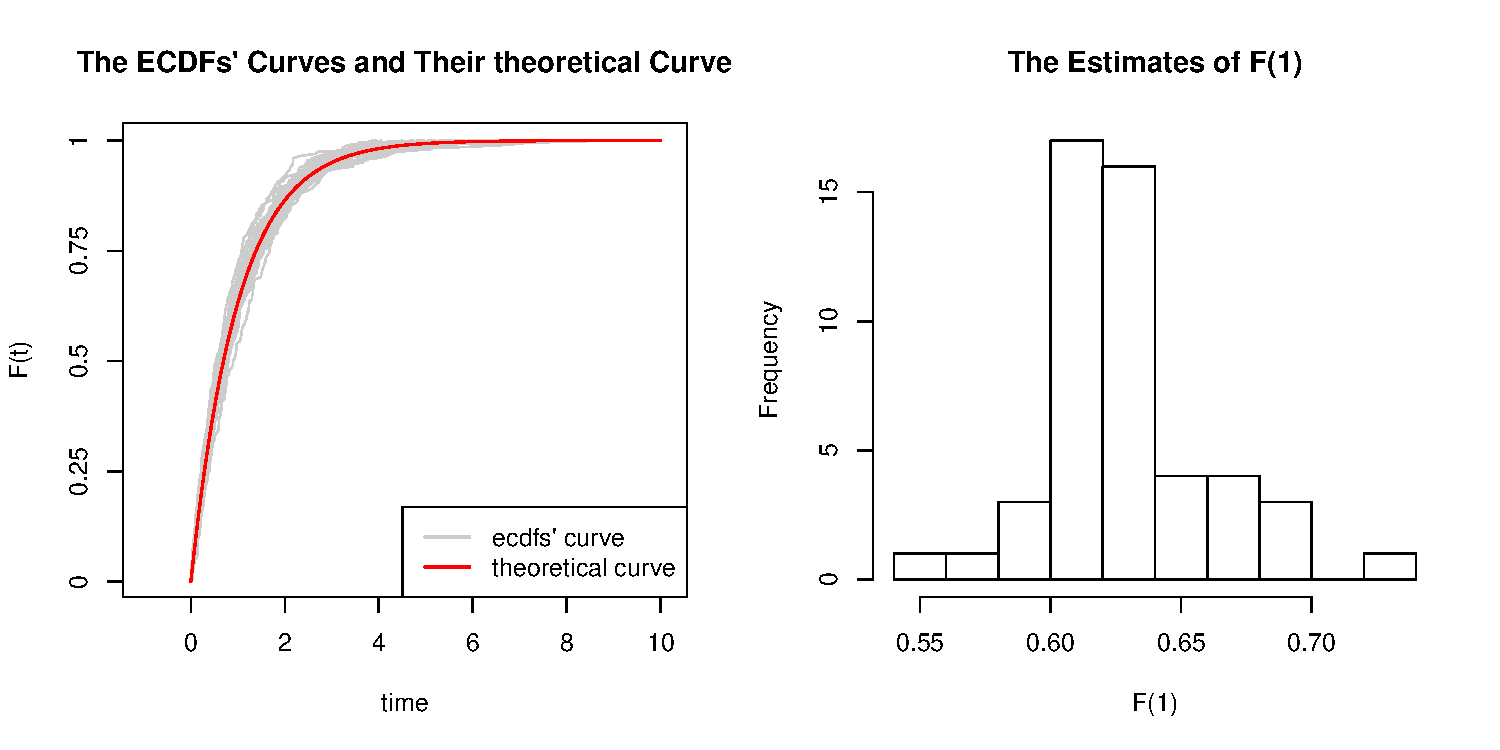
\includegraphics[width = 6 in]{3_10_ab.pdf}
		\end{figure}
%	\end{center}
		\begin{figure}[h]
			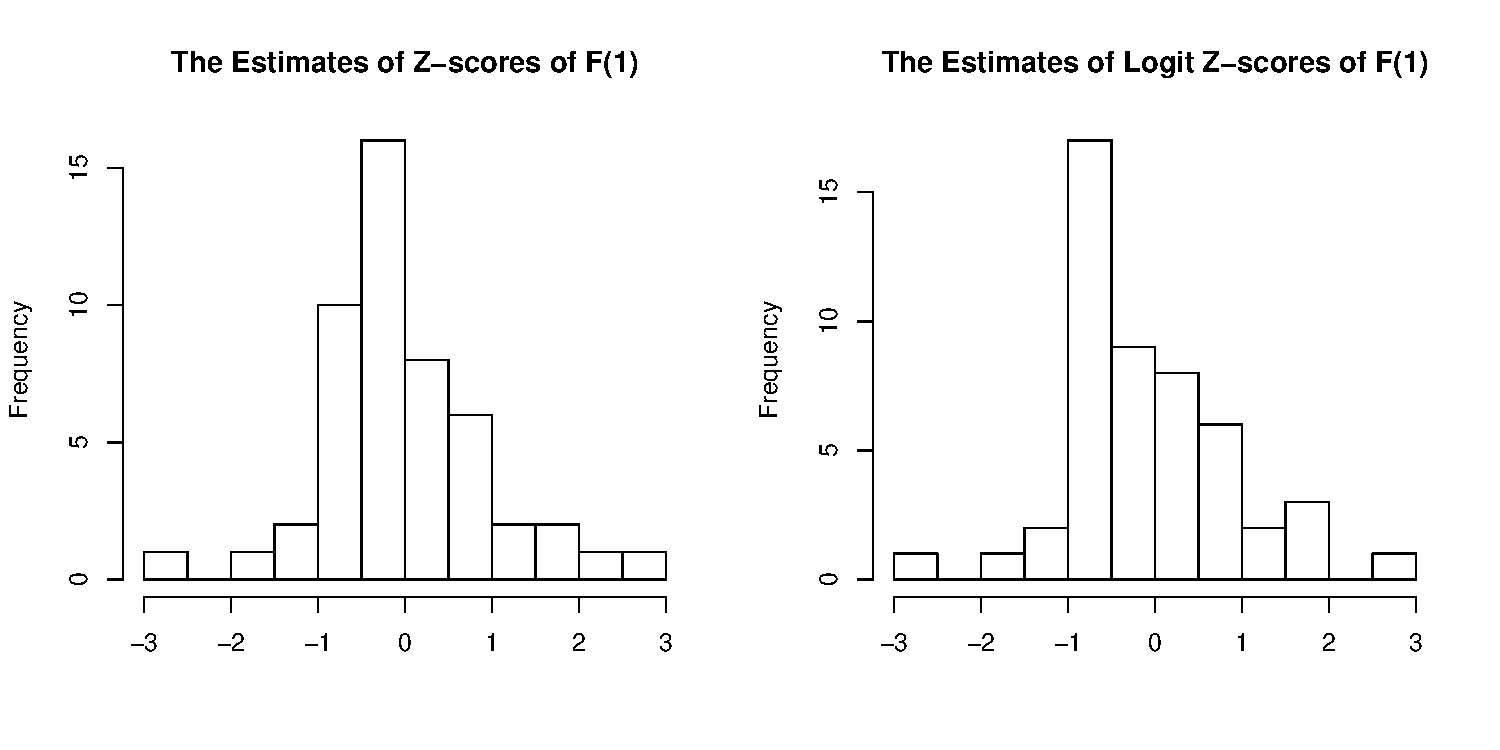
\includegraphics[width = 6 in]{3_10_cd.pdf}
		\end{figure}		
	}
	\newpage
	\item[$n$]{ $=20$
		\begin{figure}[h]
			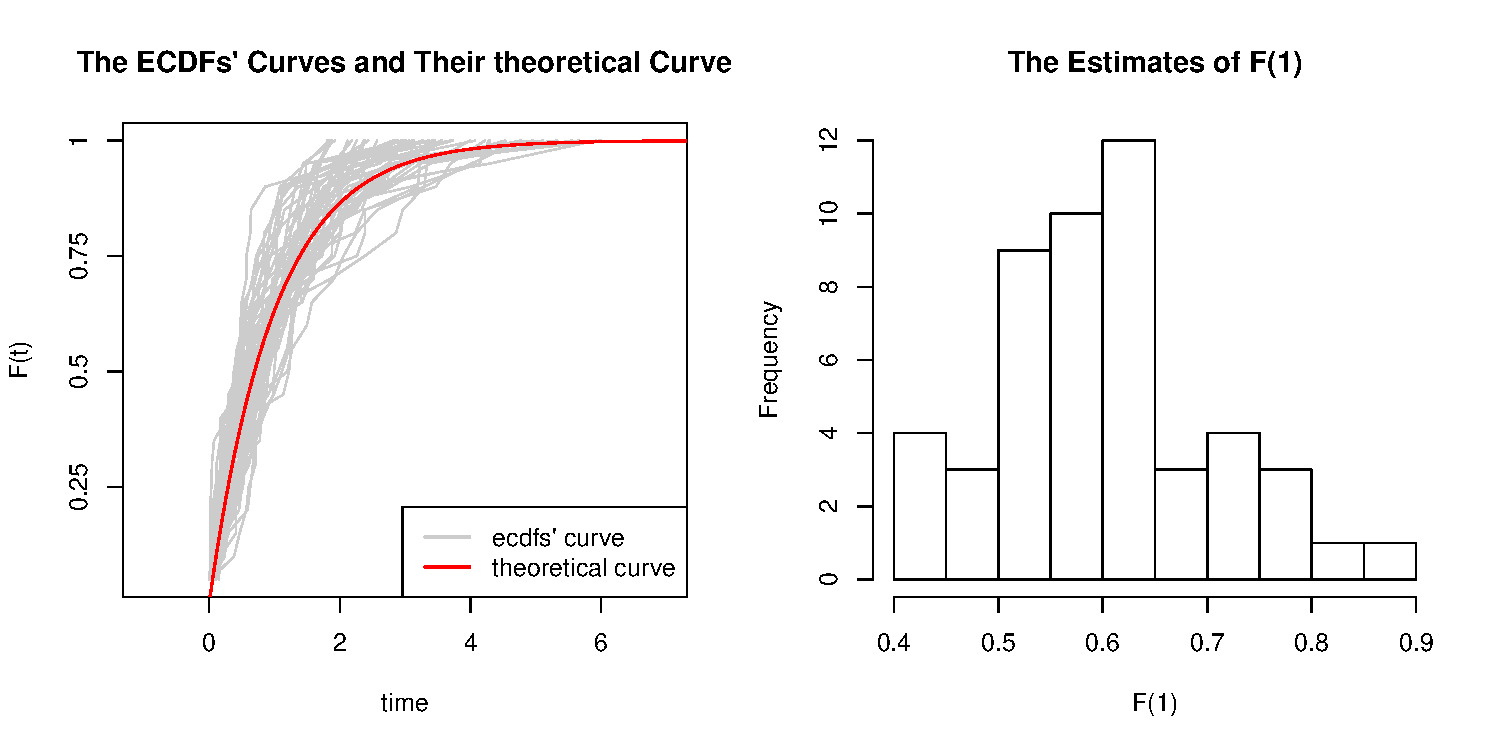
\includegraphics[width = 6 in]{3_11_1.pdf}
		\end{figure}		
		\begin{figure}[h]
			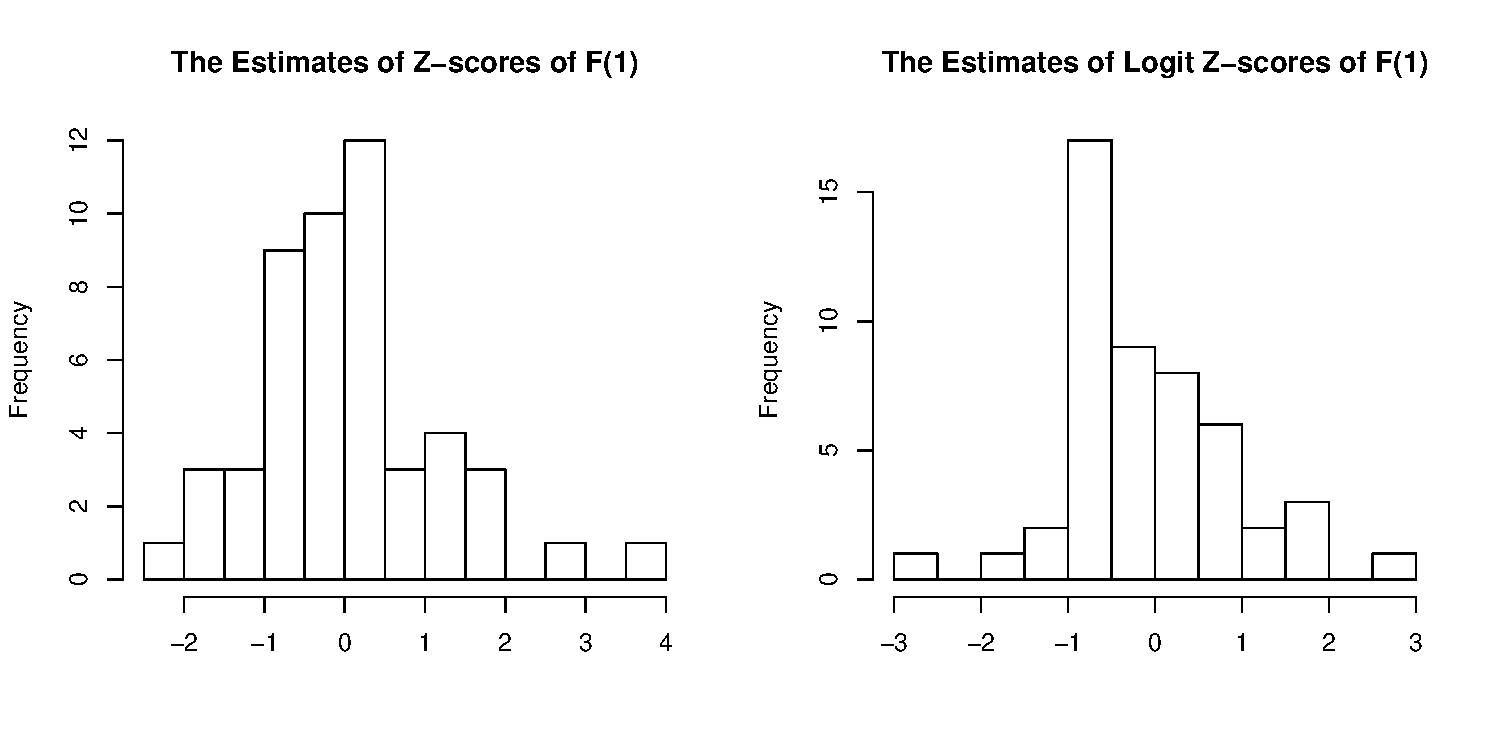
\includegraphics[width = 6 in]{3_11_2.pdf}
		\end{figure}			
	}
\end{itemize}

\qquad The ECDFs converge to the theoretical curve as the sample size $n$ increases. Also, $\widehat{F}(1)$, $Z_{\widehat{F}(1)}$ and $Z_{logit\left(\widehat{F}(1)\right)}$ with $n=200$ are more like normal distributions than those with $n = 20$.


\newpage
%----------------------------------------------------------------------------------------
%	3.12
%----------------------------------------------------------------------------------------
3.12

		\begin{table}[h]
			\begin{center}
			\begin{tabular}{ccrrrrrr}
				$i$  	& 	$t_i$ 	&  	$\widehat{F}(t_i)$ & 
				$\widehat{se}_{\widehat{F}(t_i)}$  & $Logit\ C.I._L$ & $Logit\ C.I._U$  & $Simu\ C.I._L$ & $Simu\ C.I._U$\\ \hline
					1 & 2500 & 0.0357 & 0.0351  & 0.0050  & 0.2142  & 0.0014  & 0.4933 \\
					2 & 3000 & 0.0714 & 0.0487  & 0.0179  & 0.2448  & 0.0072  & 0.4478 \\
					3 & 3500 & 0.1429 & 0.0661  & 0.0547  & 0.3245  & 0.0286  & 0.4855 \\
					4 & 3600 & 0.1786 & 0.0724  & 0.0763  & 0.3638  & 0.0427  & 0.5145 \\
					5 & 3700 & 0.2143 & 0.0775  & 0.0996  & 0.4021  & 0.0585  & 0.5447 \\
					6 & 3800 & 0.2500 & 0.0818  & 0.1241  & 0.4395  & 0.0759  & 0.5750 \\
			\end{tabular}
			\end{center}
		\end{table}

		\begin{figure}[h]
			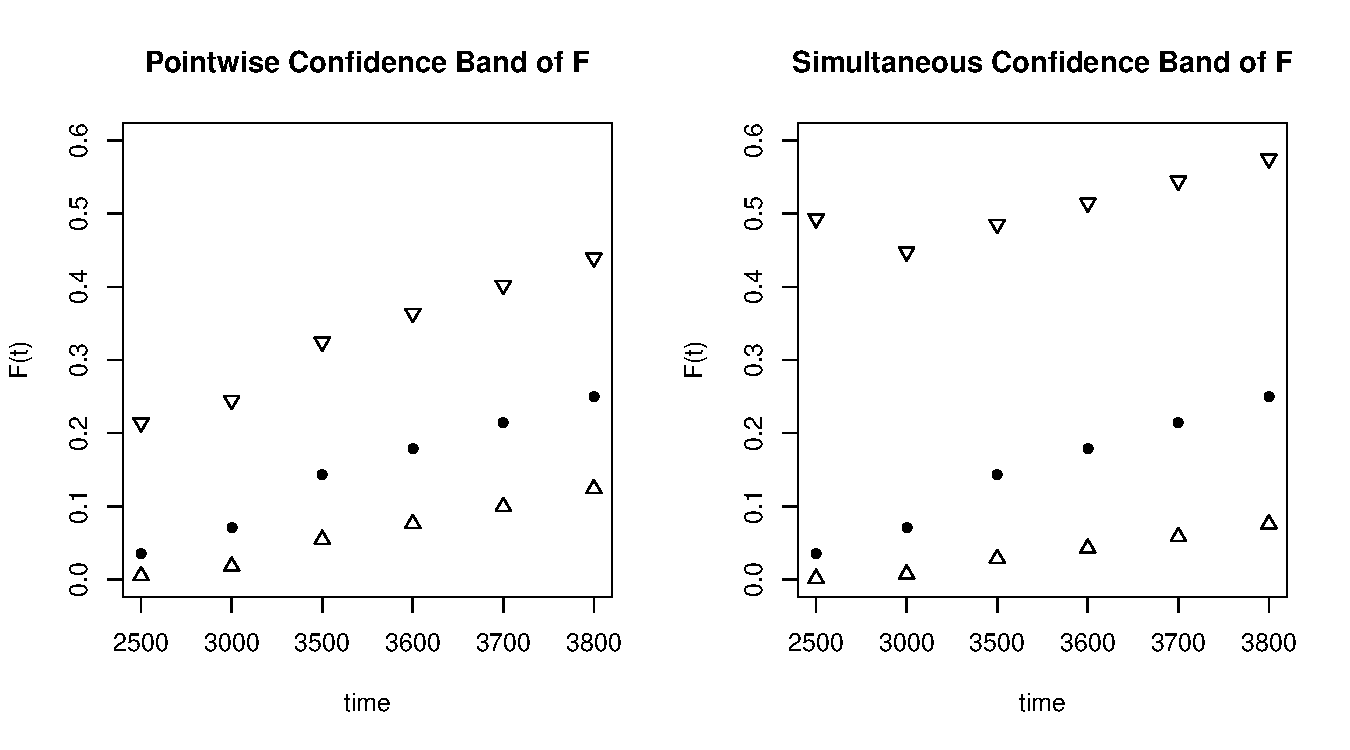
\includegraphics[width = 6 in]{3_12_de.pdf}
		\end{figure}		

\begin{itemize}

	\item[(a)]{
		The experiment checked at particular time points, this set is a multiply-censored data. 
	}
	\item[(b)]{(c) (d) (e)\\
		The answer is shown in the table and the figures above.		
	}
	\item[(f)]{
		Pointwise confidence interval is for only "one" particular $t_i$ .Simultaneous confidence band quantify sampling uncertainty simultaneously over a range of  $t_i$'s, $t_i \in (a, b)$. Therefore, simultaneous confidence band is wider than pointwise one at the same level.
	}
	
\end{itemize}

\newpage
%----------------------------------------------------------------------------------------
%	3.17
%----------------------------------------------------------------------------------------
3.17
		\begin{table}[h]
			\begin{center}
			\begin{tabular}{ccrrrr}
				$i$  	& 	$t_i$ 	&  	$\widehat{F}(t_i)$ & 
				$\widehat{se}_{\widehat{F}(t_i)}$  & $C.I._L$ & $C.I._U$ \\ \hline
				1  &1 &0.0133 &0.0066 &0.0050 &0.0350 \\
				2  &2 &0.0384 &0.0128 &0.0198 &0.0730 \\
				3  &3 &0.0582 &0.0187 &0.0307 &0.1076

			\end{tabular}
			\end{center}
		\end{table}

%----------------------------------------------------------------------------------------
%	3.19
%----------------------------------------------------------------------------------------
3.19

		\begin{table}[h]
			\begin{center}
			\begin{tabular}{ccrrrr}
				$i$  	& 	$t_i$ 	& $p(t_i)$ &	$\widehat{F}(t_i)$ & $C.I._L$ & $C.I._U$ \\ \hline
				1 & 25  &0.5798 &0.5798 &0.5081 &0.6483 \\
				2 & 50  &0.5316 &0.8032 &0.7402 &0.8539 \\
				3 & 75  &0.4595 &0.8936 &0.8409 &0.9303 \\
				4 &100 &0.3500 &0.9309 &0.8846 &0.9594
			\end{tabular}
			\end{center}
		\end{table}

		\begin{figure}[h]
			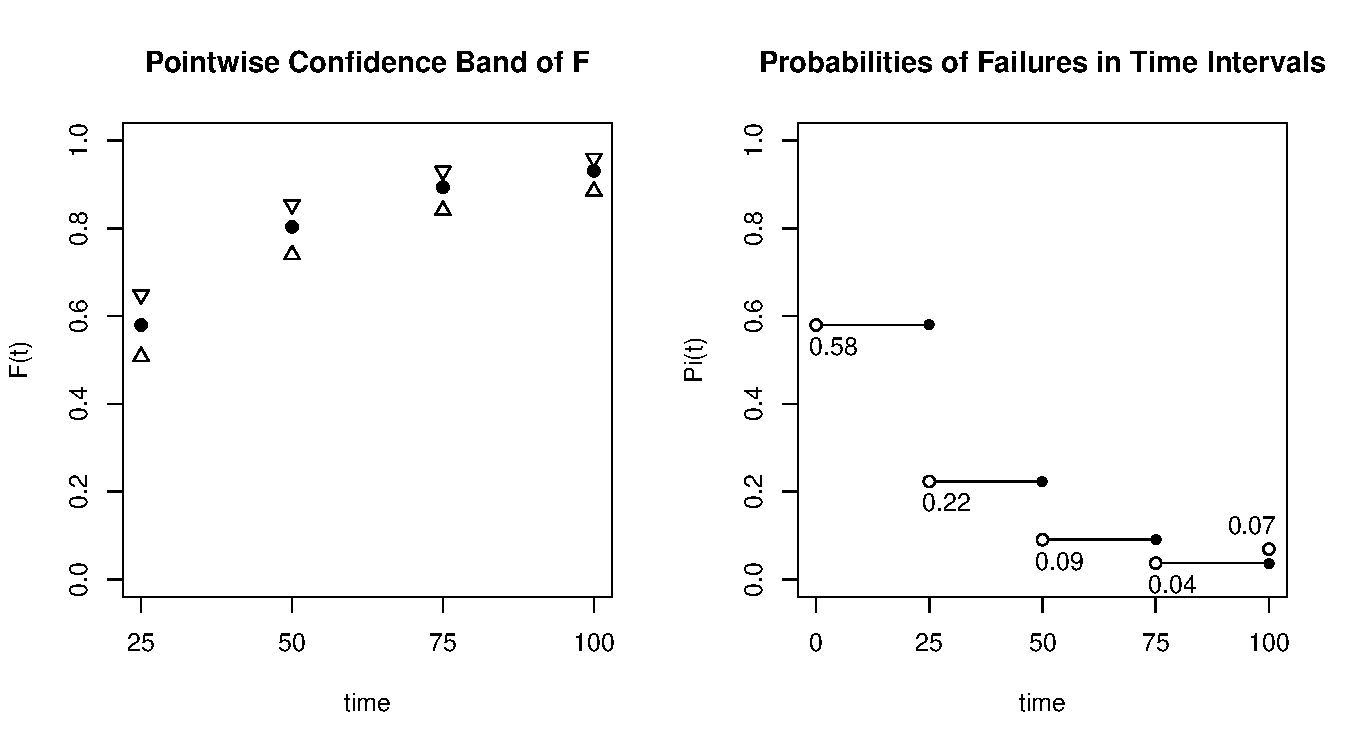
\includegraphics[width = 6 in]{3_19.pdf}
		\end{figure}		

\begin{itemize}
	\item[(a)]{(b) \ (c) \ (d)\\
		The answer is shown in the table and the figures above.
	}
	\item[(e)]{
		The failure rate was high initially, however it decreased as the time went by.
	}
\end{itemize}

\newpage
%----------------------------------------------------------------------------------------
%	3.21
%----------------------------------------------------------------------------------------
3.21 \qquad All the answers are shown in the table and the figure.
		\begin{table}[h]
			\begin{center}
			\begin{tabular}{ccrrrr}
				$i$  	& 	$t_i$ 	&  	$\widehat{F}(t_i)$ & 
				$\widehat{se}_{\widehat{F}(t_i)}$  & $C.I._L$ & $C.I._U$ \\ \hline
 1   & 50     &0.0153    &0.0152 &0.0029 &0.0752 \\
 2   &100    &0.0153    &0.0152 &0.0029 &0.0752 \\
 3   &150    &0.0330    &0.0230 &0.0103 &0.1006 \\
 4   &200    &0.1089    &0.0421 &0.0564 &0.1997 \\
 5   &250    &0.1296    &0.0460 &0.0708 &0.2254 \\
 6   &300    &0.1511    &0.0496 &0.0861 &0.2516 \\
 7   &350    &0.1734    &0.0531 &0.1024 &0.2784 \\
 8   &400    &0.2679    &0.0647 &0.1754 &0.3864 \\
 9   &500    &0.3706    &0.0732 &0.2600 &0.4967 \\
10  &550    &0.4266    &0.0767 &0.3076 &0.5547 \\
11  &600    &0.4839    &0.0790 &0.3579 &0.6121 \\
12  &650    &0.5126    &0.0796 &0.3837 &0.6399 \\
13  &700    &0.5717    &0.0802 &0.4378 &0.6958 \\
14  &750    &0.6023    &0.0801 &0.4663 &0.7241 \\
15  &850    &0.6940    &0.0772 &0.5551 &0.8049 \\
16  &900    &0.6940    &0.0772 &0.5551 &0.8049 \\
17  &1000  &0.6940    &0.0772 &0.5551 &0.8049 \\
18  &1050  &0.7323    &0.0764 &0.5903 &0.8386 \\
19  &1100  &0.7323    &0.0764 &0.5903 &0.8386 \\
20  &1150  &0.7323    &0.0764 &0.5903 &0.8386 \\
21  &1200  &0.7992    &0.0815 &0.6332 &0.9018 \\
22  &1350  &0.8661    &0.0771 &0.6844 &0.9508 \\
23  &1550  &0.9331    &0.0610 &0.7364 &0.9858 \\
24  &1700  &1.0000    &$NA$   &$NA$   & $NA$   
			\end{tabular}
			\end{center}
		\end{table}

		\begin{figure}[h]
			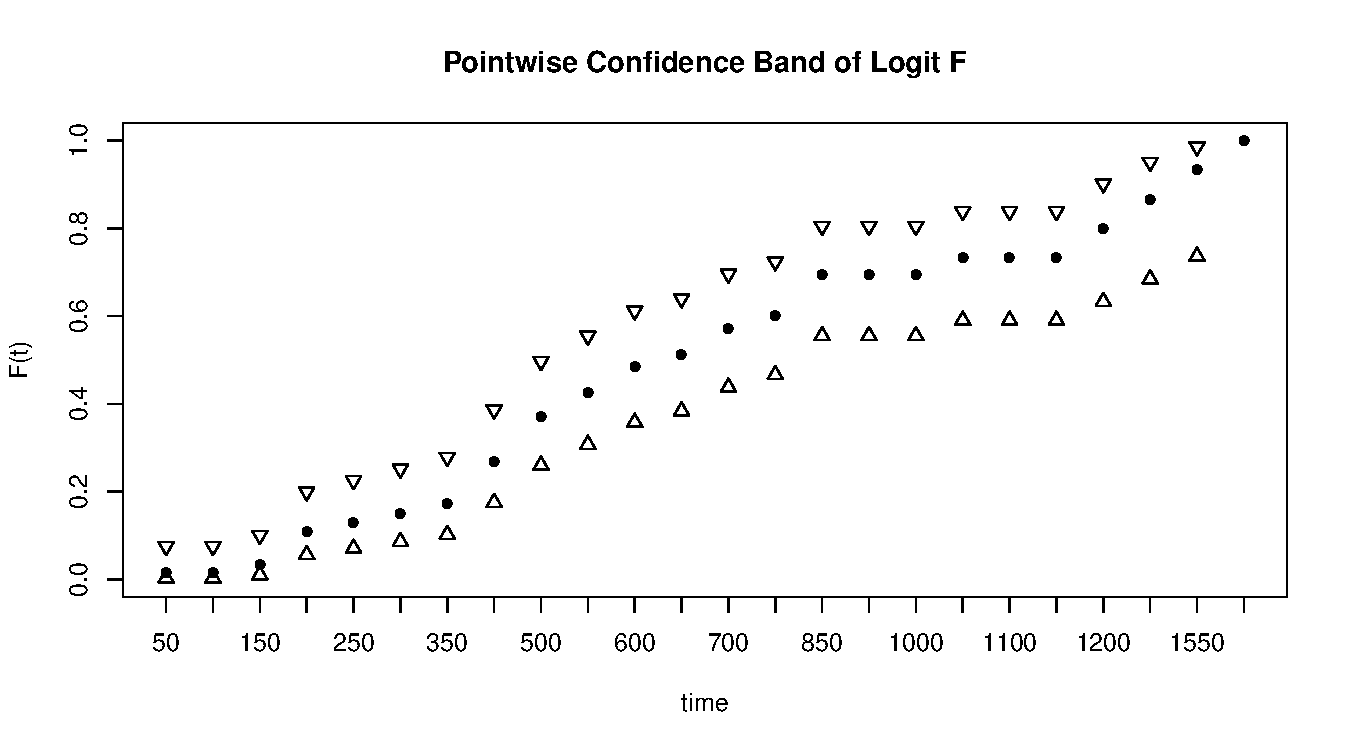
\includegraphics[width = 6 in]{3_21.pdf}
		\end{figure}		
\newpage
%----------------------------------------------------------------------------------------
%	3.22
%----------------------------------------------------------------------------------------
3.22

\begin{itemize}
	\item[(a)]{
		\begin{align*}
			L(\pi)	&=	\pi_{1}^{d_1}\cdot\pi_{2}^{d_2}\cdots\pi_{m}^{d_m}\cdot(\pi_2+\cdots+\pi_{m+1})^{r_1}\cdot(\pi_3+\cdots+\pi_{m+1})^{r_2}\cdots(\pi_m+\pi_{m+1})^{r_{m-1}}\cdot\pi_{m+1}^{r_m}\\
				&=	\pi_{1}^{d_1}\cdot\pi_{2}^{d_2}\cdots\pi_{m}^{d_m}\cdot S(t_1)^{r_1}\cdot S(t_2)^{r_2}\cdots S(t_m)^{r_m}
		\end{align*}
	}
	
	\item[(b)]{
		\begin{align*}
			\because\ \ p_i 	=& 	\frac{\pi_i}{S(t_{i-1})}\ \text{, } \forall \ i = 1, 2, \dots, m \\
			L(p)			=&	\left( p_1\cdot S(t_{0})\right)^{d_{1}}\cdot\left( p_2\cdot S(t_{1})\right)^{d_{2}}\cdots\left( p_m\cdot S(t_{m-1})\right)^{d_{m}}\cdot S(t_1)^{r_1}\cdot S(t_2)^{r_2}\cdots S(t_m)^{r_m}\\
						=&	p_{1}^{d_{1}}\cdot p_{2}^{d_{2}}\cdots p_{m}^{d_{m}}\cdot  S(t_1)^{r_1+d_2}\cdot S(t_2)^{r_2+d_3}\cdots S(t_{m-1})^{r_{m-1}+d_m}\cdot S(t_m)^{r_m}\\
						=&	p_{1}^{d_{1}}\cdot p_{2}^{d_{2}}\cdots p_{m}^{d_{m}}\cdot (1-p_1)^{r_1+d_2}\cdot \left((1-p_1)(1-p_2) \right)^{r_2+d_3}\cdots \\
						  & \cdots \left((1-p_1)(1-p_2)\cdots(1-p_{m-1}) \right)^{r_{m-1}+d_m}\cdot   \left((1-p_1)(1-p_2)\cdots(1-p_{m}) \right)^{r_m} \\
						=&	p_{1}^{d_{1}}\cdot p_{2}^{d_{2}}\cdots p_{m}^{d_{m}}\cdot (1-p_1)^{r_m+\sum_{i = 1}^{m-1}(d_{i+1}+r_i)}\cdot (1-p_2)^{r_m+\sum_{i = 2}^{m-1}(d_{i+1}+r_i)}\cdots \\
						  &	\cdots(1-p_{m-1})^{r_m+\sum_{i = {m-1}}^{m-1}(d_{i+1}+r_i)}\cdot(1-p_m)^{r_m}\\
						=& 	p_{1}^{d_{1}}\cdot p_{2}^{d_{2}}\cdots p_{m}^{d_{m}}\cdot (1-p_1)^{n_1-d_1}\cdot (1-p_2)^{n_2-d_2}\cdots (1-p_m)^{n_m-d_m}\\
						=&	\prod_{j=1}^mp_j^{d_j}(1-p_j)^{n_j-d_j}
		\end{align*}
	}
	
	\item[(c)]{
		\begin{align*}
				&log\left( L(p) \right) = \sum_{j=1}^m\left( d_jlog(p_j)+(n_j-d_j)log(1-p_j)\right)\\
	\text{Let,\ \ \ }&\frac{\partial log\left( L(p) \right)}{\partial p_j} =\frac{d_j}{p_j} - \frac{n_j-d_j}{1-p_j}=0\ \ \ \Rightarrow\ \  p_j = \frac{d_j}{n_j}\\
	\because\ \   &	\left. \frac{\partial^2 log\left( L(p) \right)}{\partial {p_j}^2} \right |_{p_j = \frac{d_j}{n_j}} <0 \text{\ \ \ \ \ \ }\therefore \widehat{p}_j = \frac{d_j}{n_j}
		\end{align*}
	}
	
	\item[(d)]{
		\begin{align*}
				&	S(t_i) = \prod_{j=1}^i(1-p_j)\ \ \Rightarrow	\ \ log\left( S(t_i) \right) = \sum_{j = 1}^i log(1-p_j)= \sum_{j = 1}^i log(q_j)	\\
	\Rightarrow\ \ 	&	\frac{1}{S(t_i)}\cdot\frac{\partial S(t_i)}{\partial q_j} = \frac{1}{q_j}\ \ \Rightarrow\ \ \frac{\partial S(t_i)}{\partial q_j} = \frac{S(t_i)}{q_j}\\
	\because\ \ 	&	\widehat{S}(t_i) \approx S(t_i)+\sum_{j=1}^i\left.\frac{\partial S(t_i)}{\partial q_j}\right |_{q_j}(\widehat{q}_j-q_j) = S(t_i)+\sum_{j=1}^i\frac{\partial S(t_i)}{\partial q_j}(\widehat{q}_j-q_j) \\
	\Rightarrow\ \ 	&	Var\left( \widehat{S}(t_i)\right) = \sum_{j=1}^{i} \left( \frac{\partial S(t_i)}{\partial q_j} \right)^2Var(\widehat{q}_j)=\sum_{j=1}^{i} \left( \frac{\partial S(t_i)}{\partial q_j} \right)^2Var(1-\widehat{p}_j)\\
				&=	\sum_{j= 1}^i\left( \frac{\partial S(t_i)}{\partial q_j} \right)^2Var(\widehat{p}_j) = \sum_{j= 1}^i\left( \frac{\partial S(t_i)}{\partial q_j} \right)^2\frac{p_j(1-p_j)}{n_j}\\
				&=	\left( S(t_i) \right)^2\sum_{j= 1}^i \left( \frac{1}{1-p_j}\right)^2 \frac{p_j(1-p_j)}{n_j} = \left( S(t_i) \right)^2\sum_{j= 1}^i \frac{p_j}{n_j(1-p_j)}\\
	\therefore	\ \ 	&	\widehat{Var}\left( \widehat{S}(t_i) \right)= \left( S(t_i) \right)^2\sum_{j= 1}^i \frac{\widehat{p}_j}{n_j(1-\widehat{p}_j)}
		\end{align*}
	}
\end{itemize}
%----------------------------------------------------------------------------------------

\end{document} \\